\section{Polymorphism}
\label{sec:polymorphyism}

Polymorphism is the ability of an entity to show diferent shapes or
forms. In biology, polymorphic animals can exist in a variety of
different forms, e.g.~male and female animals, or different blood
types. In materials science, polymorphic materials can exist in a
variety of different crystaline configurations (e.g.~calcite and
aragonite). 

In computer science, polymorphism appears at many levels. In
Programming in Java, we are mainly interested in two types of polymorphism:
polymorphic classes and polymorphic methods. The former is usually
referred to as \emph{generic types}, while the latter is usually
called \emph{method overloading}. 

\section{Generic types/classes}
\label{sec:generic-types}

A generic type or generic class
is a complex type that can be combined with other
different types to produce a new type. 
The most common application of generic types is for
``container'' classes like lists, stacks, and queues. 

When we were creating our own dynamic classes in previous weeks, they
were usually attached to a type: lists of strings, stacks of integers,
etc. 

\begin{verbatim}
    // Part of a String List              // Part of an IntegerList
    public class StringNode {             public class IntegerNode {
        private String value;                 private Integer value;
        private StringNode next;              private IntegerNode next;
        // ...                                // ...
    }                                     }
\end{verbatim}

This seems a bit like code repetition. A \emph{generic class}, on the 
other hand, could work in the same with more than one
type, saving the programmer from the hassle of having different but very
similar types (e.g. stacks) for each different type of data they want
to use (i.e.~string stacks, integer stacks, patient stacks, etc). 

\subsection{Using generic classes}
\label{sec:using-gener-class}

A generic class is very similar to a normal class. The only
difference ---but it is a crucial one--- is that it uses one or more
\emph{type parameter} to indicate that it needs another type to be
fully declared. Type parameters
are specified in low quotes (``$<$'', ``$>$''). Let's see an
example of a generic interface, a stack (JavaDoc comments removed for
brevity): 

\begin{verbatim}
    public interface Stack<T> {
        void push(T object);
        T pop();
    }
\end{verbatim}

The type parameter \verb+T+ represents a type to be determined when the
interface \verb+Stack<T>+ is used. For example, we could declare a
\verb+Stack<String>+ or a \verb+Stack<Integer>+ (see below). 

If we wanted to implement this interface using arrays, it could look
like this (comments removed for brevity): 

\begin{verbatim}
    public class ArrayStack<T> implements Stack<T> {
        private T[] contents;
        private int headIndex; 

        public void push(T newElement) {
            contents[headIndex] = newElement;
            headIndex++;
        }
        public T pop() {
            if (headIndex == 0) {
                return null;
            }
            headIndex--;
            T result = contents[headIndex];
            contents[headIndex] = null;
            return result;
        }
        // ... constructor and other methods would be here ...
    }
\end{verbatim}

As you can see, there are two main differences between a normal class
and a generic class (and their methods): 

\begin{itemize}
\item The name of the class is extended to include the type, by using
  a type parameter in low quotes. Capital \verb+T+ (for ``type'') is a common
  name for type parameters. By convention type parameters are
  usually capital single letters (T for ``type'', K for ``key'', 
  V for ``value'', etc), but any valid identifier can be
  used.
\item The variable type can be used in every place where a type
  (simple or complex) should be: parameter types, return types, and
  for declaring new variables. 
\end{itemize}

How are generic interface and classes used? Look at this code:

\begin{verbatim}
    // ...
    Stack<Integer> myNumberStack = new ArrayStack<Integer>();
    Stack<String> myStringStack = new ArrayStack<String>();
    myNumberStack.push(1);
    myStringStack.push("Test string!");
    // ...
\end{verbatim}

As you can see, the same generic interface and generic class can be used to handle
different specific interfaces/classes, i.e.~stacks 
of integers and strings in this case. Generic types
must be based on complex types (classes), not simple types. Boxed
types are useful if you need a generic type based on one of the
primitive (i.e.~simple types). 
This is why the example uses a \verb+Stack<Integer>+; if you try
to create a \verb+Stack<int>+, Java will complain. 

\subsection{Restricting generic types}
\label{sec:restr-gener-types}

There are situations in which you want to create a generic type that
can only be combined with some specific types.
For example, you
may want to use a list of \verb+Person+ in your program, but you do
not want lists of string or hospitals appearing in your code from other
modules. 

Restricting the type is easy and can be done in more than one way. For
now, we will look at just one way of doing it by means of
interfaces. Look at this example:

\begin{verbatim}
    public interface PersonList<P extends Person> {
        void push(P object);
        P pop();
    }
\end{verbatim}

In this case, we are using P instead of T for the type parameter to
make it clearer that it must be a Person, not just any type. Note that
the keyword to retrict the type parameter is \verb+extends+, not
\verb+implements+. The
compiler knows that any type that we specify for \verb+PersonList<P>+
must be a class that extends/implements the interface \verb+Person+. Therefore, we will be
able to create a \verb+PersonList<KidPerson>+ but not a
\verb+PersonList<Integer>+. If we try to do the latter, Java will
complain. 

\subsection{Type wildcards}
\label{sec:type-wildcards}

Generic classes can also be used in a generic way (no pun
intended). For example, we may want to write a method that takes a
generic class inside a non-generic class, as in this example, where a
\verb+School+ class has a method that always returns the first element
of a list, regardless of it being a list of students, of teachers, or of
homework assignments: 

\begin{verbatim}
    public class School {
        // ...
        public T returnFirstElement(List<T> stack) {
            return stack.get(0); 
        }
        public int returnElementCount(List<T> stack) {
            return stack.size();
        }
        // ... more methods here
    }
\end{verbatim}

If you try to compile this method, the compiler will complain because
it does not know what the type parameter T is. There are three ways of
solving this problem. First, we could make School a generic class: 

\begin{verbatim}
    public class School<T> {
        // ...
\end{verbatim}

This is a bad idea. Classes should not be made generic unless there is
a reason for it. Generics add an additional level of complexity in the
code that must be balanced with some clear benefit, as in the case of
container classes (lists, stacks, trees, maps, etc). Another
possibility is to generify only the method
\verb+returnFirstElement()+: 

\begin{verbatim}
    public class School {
        // ...
        public <T> T returnFirstElement(List<T> stack) {
            return stack.get(0); 
        }
        // ... more methods here
    }
\end{verbatim}

This is slightly better because it keeps the generics more
contained, i.e.~restricted to the method. 

If the method returns a generified type, restricting generics to the
methods is the best
we can do. However, if the return type is not generic, 
we can use an even simpler notation using type wildcards: 

\begin{verbatim}
    public class School {
        // ...
        public int returnElementCount(List<?> stack) {
            return stack.size();
        }
        // ... more methods here
    }
\end{verbatim}

A type wildcard (i.e.~a question mark) means that the generic
type can be specified with any other type. Wildcards can be restricted
if necessary: 

\begin{verbatim}
    public class School {
        // ...
        public int returnElementCount(List<? extends Person> stack) {
            return stack.size();
        }
        // ... more methods here
    }
\end{verbatim}

In this case, the method will accept a list of any type as long as the
type is a \verb+Person+. 

% Maybe add something here about PECS? Next year!
%
% http://www.ibm.com/developerworks/java/library/j-jtp07018/index.html#3.0
% 
% http://stackoverflow.com/questions/2248390/java-generics-collections-max-signature-and-comparator/2248503#2248503
% 
% http://stackoverflow.com/questions/2723397/java-generics-what-is-pecs 


\subsection{Conclusion}
\label{sec:conclusion-2}

Generic classes are one of the main types of polymorphism present in
Java. They enable programmers to combine one class with several other
classes, by using type parameters. 

Generic classes are, therefore, a way of reusing code and/or avoiding
code repetition (remember the DRY principle: Don't Repeat Yourself). 
There is no need to create a list of integers, a list of
strings, and a list of books. It is better to create a generic list
that can be combined with any type, and then combine it with integers,
string, books, or any other type as needed. The drawbacks of generic
classes is that they are slightly more verbose (i.e.~the programmer
needs to write more) and that they can become very confusing if
abused, e.g. when generic classes of generic classes of generic
classes are employed. 

A full description of generics in Java, how they are implemented
internally, and the full list of possibilities and caveats, is beyond
the scope of this course. As a rule of thumb, use generics sparingly in
Java and do not use generics of generics. Your brain will thank you. 


\section{Method overloading}
\label{sec:method-overloading}

Another very common form of polymorphism is \emph{method
  overloading}. This is just a fancy name to say that a method can
receive different parameters. We have seen several examples already,
such as the method \verb+substring+ of class \verb+String+. This
method can take either one or two \verb+int+ parameters; depending on
the number of arguments, the behaviour is different. 

\begin{verbatim}
    // ...
    String str = "This is some text";
    System.out.println(str.subString(8));    // prints "some text"
    System.out.println(str.subString(8,12)); // prints "some"
    // ...
\end{verbatim}

A method in Java is defined by its name and the types and positions of
its parameters; therefore, strictly speaking, \verb+substring(int)+ is
a different method from \verb+substring(int,int)+ and it is not a
problem if both are present in class \verb+String+. The following
methods, however, do have the same \emph{signature} and there can be
only one version in each class: 

\begin{verbatim}
    // Same method! Cannot be in same class.
    String myMethod(int first, int second, String message);
    String myMethod(int start, int end, String txt);
\end{verbatim}

Remember that the names of the parameters are not important: only their types and
positions. Note that the return type is not part of the signature
either, so we cannot have two methods with the same name and
parameters but different return types. 

\begin{verbatim}
    // Same method! Cannot be in same class.
    int myMethod(int first, int second, String message);
    void myMethod(int first, int second, String message);
\end{verbatim}

\paragraph{Method overloading without repeating code}
\label{sec:meth-overl-with}

One thing that a programmer must bear in mind when method overloading
is used is not to repeat code. For example, the following overloaded
method repeats code unnecesarily: 

\begin{verbatim}
    public void printAverage(double d1, double d2) {
         double result = 0.5 * (d1 + d2);
         System.out.println("The average is: " + result);
    }
    public void printAverage(double d1, double d2, String msg) {
         double result = 0.5 * (d1 + d2);
         System.out.println(msg + result);
    }
\end{verbatim}

There is repeated code among both versions of the method. In this
trivial example this is just one line, but in a more serious program
this could be some non-trivial algorithm that is repeated, and we know
that code repetition must be avoided. 

Avoiding this kind of code repetition is easy by making the more
specific version of the method call the more general version, as in
the code below: 

\begin{verbatim}
    public void printAverage(double d1, double d2) {
         printAverage(d1, d2, "The average is: ");
    }
    public void printAverage(double d1, double d2, String msg) {
         double result = 0.5 * (d1 + d2);
         System.out.println(msg + result);
    }
\end{verbatim}

This is how we can have multiple polymorphic versions of the same
method without any repetition of code. Remember: Don't Repeat
Yourself. 

\section{Upcasting and downcasting}
\label{sec:upcasting}

There is a third type of
polymorphism (of sorts) in Java that is simpler but also very
important. 
We have
already seen how it works, although we have not used its proper name
until now.
%We are already familiar with \emph{upcasting}, although we have not
%called it like that. 
We have been using it every time we have declared
a variable by using an interface or a superclass: 

\begin{verbatim}
    List patientList;
    patientList = new ArrayPatientList();
\end{verbatim}

We know that it is good practice to work with interface names for our
data types, rather than to use the class names directly. Using interfaces
allows programmers to abstract themselves from all the implementation details
of the class and work with just its public behaviour, i.e.~the methods
defined on the interface. This is called \emph{upcasting}, and it is similar to the
casting of simple types we have already seen; you just need to know
that, by convention, interfaces are imagined to be ``up'' and specific
classes are imagined to be ``down'' (see Figure~\ref{fig:updown}), so casting from class to
interface is up-casting. (The ``origin'' in computer science is almost
always up: the root of a tree, the interface of a class, etc). 

\begin{figure}[hbtp]
  \centering
  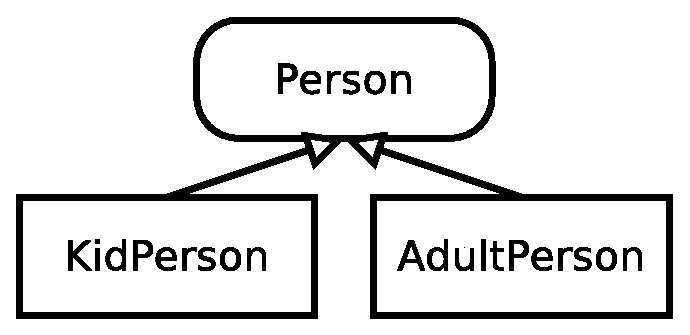
\includegraphics[height=3cm]{gfx/class_diagram-person}
  \caption{Interface Person is implemented by classes KidPerson and
    AdultPerson. By convention, the interface is represented ``up'' and
    the classes are represented ``down''.} 
  \label{fig:updown}
\end{figure}

Another useful form of upcasting is when a programmer uses an
interface as a type for a generic class: 

\begin{verbatim}
    Stack<Person> myPersonStack = new ArrayStack<Person>();
\end{verbatim}

On the left-hand side, we have a generic interface (\verb+Stack<T>+) that is made
specific by using another interface (\verb+Person+). The variable
\verb+myPersonStack+ will point to a stack that will only store
objects of classes that implement the \verb+Person+ interface
(e.g. \verb+KidPerson+, \verb+AdultPerson+, etc). 

Upcasting is a way of ``moving up to know less'', i.e.~to
intentionally forget details about the implementation so that we can
work with a simpler, more generic data type. 
Bear in mind that a real program is really complex, and therefore
reducing complexity is usually in the programmer's benefit; that
is why upcasting is so common in Java programs. 

In some rare occasions,
programmers need to do the opposite, i.e.~move down from the general
to the specific: this is called \emph{downcasting}. The syntax in this
case is very similar to the casting of simple types. Imagine that we
have a list of animals, but we knew (somehow) that all those animals
were dogs, and we wanted to make them bark. As \verb+bark()+ is a
method of \verb+Dog+ but not of \verb+Animal+ we would need to
downcast them: 

\begin{verbatim}
    public void makeThemBark(List<Animal> animals) {
        for (int i = 0; i < animals.size(); i++) {
            Animal nextAnimal = animals.get(i);
            Dog dog = (Dog) nextAnimal;
            dog.bark();
        }
    }
\end{verbatim}

Upcasting is an operation that detects errors at compile time: if the
code compiles, it will always run. This is not true of downcasting, which can
fail at \emph{runtime}, even if it compiled successfully. In the
example above, the method \verb+makeThemBark(...)+ may receive a list
of \verb+Animal+ where not all the elements are really objects of
class \verb+Dog+ (maybe there is a \verb+Cat+). When the code tries to
downcast a class into something that it is not, Java will throw a
\verb+ClassCastException+: 

\begin{verbatim}
    java.lang.ClassCastException: Cat cannot be cast to Dog
\end{verbatim}


%%% Local Variables:
%%% mode: latex
%%% TeX-master: "d12"
%%% End:
